\documentclass{article}
\usepackage[margin=1in]{geometry}
\usepackage{graphicx}
\usepackage{amsmath}
\usepackage{float}
\usepackage{tikz}
\usetikzlibrary{shapes, arrows, positioning}

\title{Power supply and control system for six MyActuator 48V RMD-X8-120 motors}
\author{Badhon Kumar}
\date{01, April 2026}

\begin{document}

\maketitle

\section{Power Supply and Control System Design}

\subsection{System Overview}
A complete power supply and control system was designed to operate six MyActuator RMD-X8-120 (48V) motors without the use of a battery bank. The system converts AC mains power into regulated DC power and distributes it safely to each motor while enabling synchronized control via a communication network.

\subsection{Power Supply Design}
The system is powered from a 110V AC mains source. Based on an estimated peak load of approximately 600 W per motor, the theoretical maximum power requirement is:

\begin{equation}
P_{total} = 6 \times 600 = 3600 \text{ W}
\end{equation}

\noindent
At 110V AC, each 1200W PSU draws approximately 11--12A at full capacity. With four PSUs operating in parallel, the total peak system current draw from the 110V AC mains will be approximately 44--48A.

\noindent
Due to this significant current draw, attempting to split the load across standard 15A or 20A wall receptacles is an unacceptable fire hazard and violates electrical safety standards. Therefore, \textbf{a dedicated 60A AC double-pole circuit breaker is strictly required} at the facility's main electrical panel. Furthermore, the AC wiring feeding the power supplies must utilize a minimum of 6 AWG copper wire to safely carry the 48A load without overheating or causing severe voltage drop.

\noindent
This modular configuration improves reliability, thermal performance, and ease of maintenance. The selected 48V AC-DC power supplies feature active current sharing (parallel function) to ensure the load is balanced equally across all four units.

\subsection{Power Distribution}
The DC outputs from the power supplies are connected to a common DC busbar. Crucially, all DC cables routing from the four PSUs to the positive and negative busbars must be of exactly equal length and gauge. Electricity follows the path of least resistance; if cable lengths differ, the PSU with the shortest cable will absorb the majority of the current load, leading to premature thermal failure.

\noindent
To handle large transient voltage spikes and absorb regenerative braking energy from the motors, a bulk capacitor bank (consisting of twelve 4700$\mu$F 63V capacitors) is placed directly on the busbars. This bank must be positioned \textbf{before} the main circuit protection. If placed after the breaker, a downstream short-circuit would bypass the breaker entirely as the capacitors discharge their stored energy directly into the fault. 

\noindent
Power is then routed through a 150A marine circuit breaker to a 6-way fuse box. Each individual motor line includes:

\begin{itemize}
    \item A 20A fuse in the 6-way distribution block.
    \item A 1000 $\mu$F / 100V low-ESR capacitor placed directly at the motor (or fuse box output). This local decoupling is mandatory to suppress violent inductive voltage spikes caused by the motors' high-frequency PWM switching, preventing electromagnetic interference (EMI) from crashing the CAN bus.
    \item Appropriately sized cables.
\end{itemize}

\subsection{Control System}
The motors are controlled using a Controller Area Network (CAN) communication protocol. A central controller (microcontroller or PC with CAN interface) sends commands to all motors through a shared CAN bus.

\noindent
All motors are connected in a daisy-chain configuration. Two 120$\Omega$ termination resistors are placed at both ends of the CAN bus to ensure signal integrity and eliminate high-frequency signal reflections.

\subsection{System Advantages}
\begin{itemize}
    \item Continuous, high-torque operation without battery dependency or degradation.
    \item Elimination of nuisance tripping and fire hazards via properly sized 60A facility infrastructure.
    \item Safe handling of short-circuits via strategic bulk-capacitor placement before the main breaker.
    \item Robust and noise-resistant CAN communication protected by local motor decoupling capacitors.
\end{itemize}

\section{Practical Design and Hardware Choice}

\begin{figure}[H]
\centering
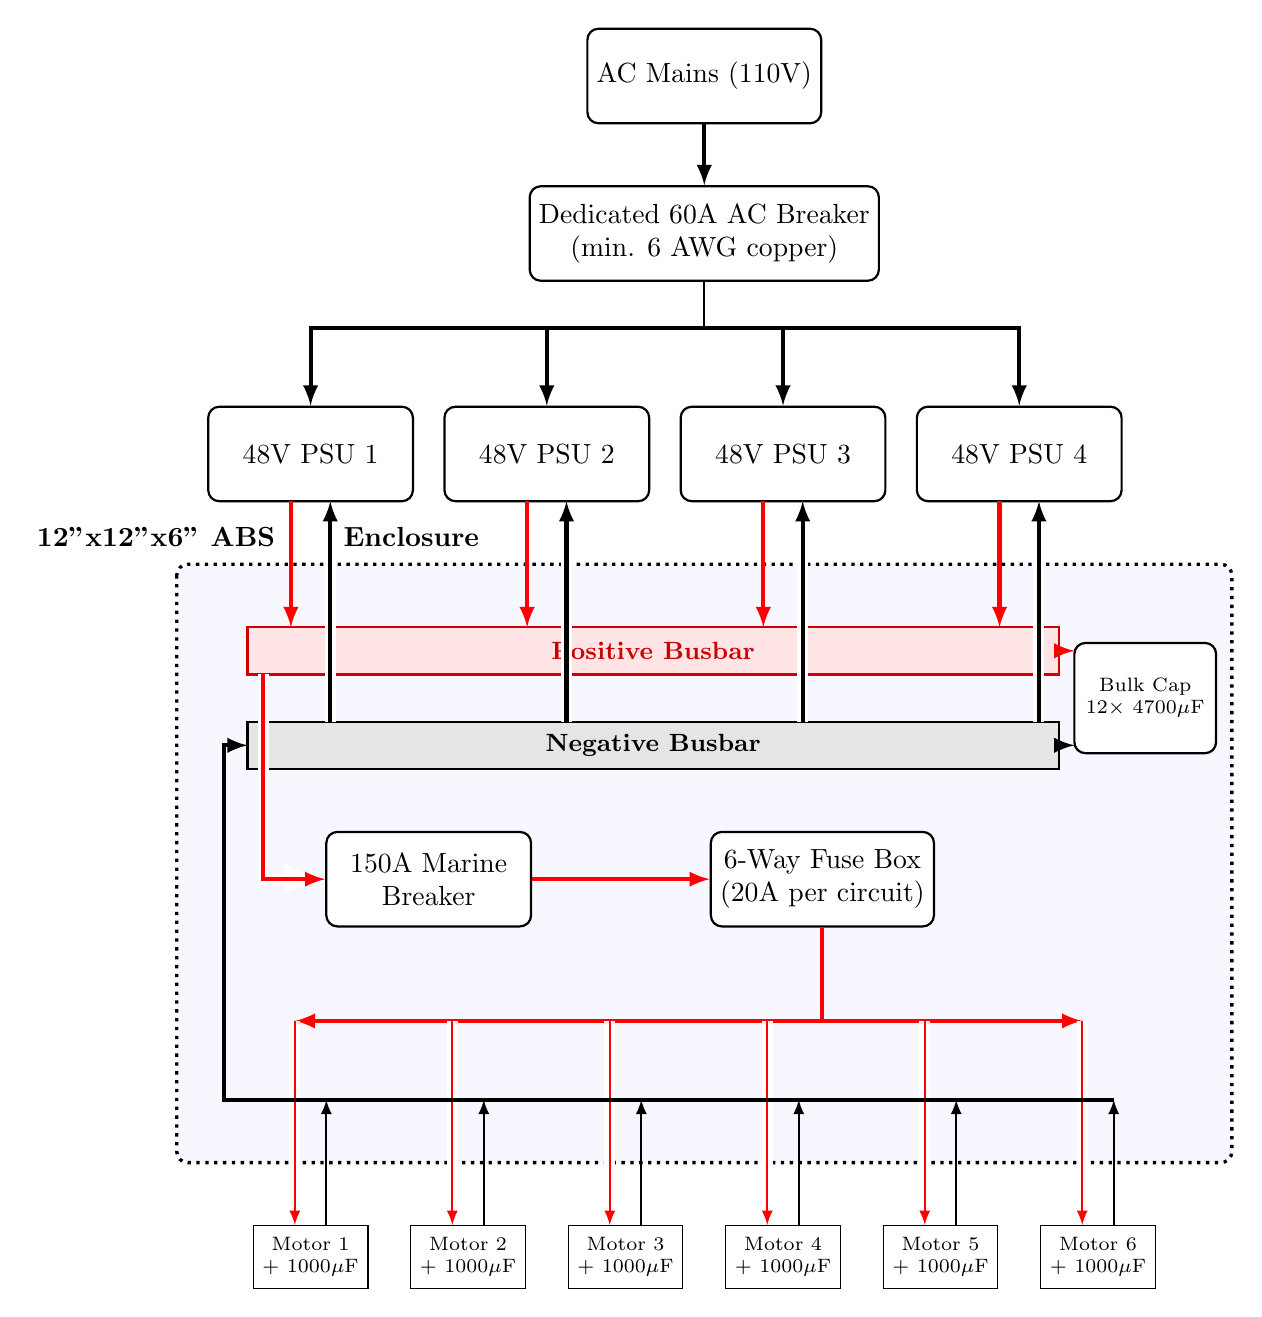
\begin{tikzpicture}[
    component/.style={rectangle, draw=black, rounded corners, align=center, minimum width=2.6cm, minimum height=1.2cm, fill=white, thick},
    smallnode/.style={rectangle, draw=black, align=center, minimum width=1.4cm, minimum height=0.8cm, font=\scriptsize, fill=white},
    heavyline/.style={draw, line width=1.5pt, -latex},
    posline/.style={draw, red, thick, -latex},
    negline/.style={draw, black, thick, -latex},
    heavyposline/.style={draw, red, line width=1.5pt, -latex},
    heavynegline/.style={draw, black, line width=1.5pt, -latex},
    jump/.style={preaction={draw, white, line width=4pt}}
]

% ─── Enclosure Boundary ──────────────────────────────────────────────
\draw[very thick, dotted, rounded corners, fill=blue!3] (-6.7, 4.8) rectangle (6.7, -2.8);
\node[anchor=south west, font=\bfseries] at (-8.6, 4.9) {12"x12"x6" ABS \hspace{6.mm} Enclosure};

% ─── AC Input (Top) ──────────────────────────────────────────────────
\node[component] (ac) at (0, 11.0) {AC Mains (110V)};
\node[component] (ac_breaker) at (0, 9.0) {Dedicated 60A AC Breaker\\(min. 6 AWG copper)};

\draw[heavyline] (ac) -- (ac_breaker);
\draw[thick] (ac_breaker.south) -- (0, 7.8);

% ─── PSUs (Pushed down for balanced spacing) ─────────────────────────
\foreach \x/\i in {-5.0/1, -2.0/2, 1.0/3, 4.0/4} {
    \node[component] (psu\i) at (\x, 6.2) {48V PSU \i};
    \draw[heavyline] (0, 7.8) -| (psu\i.north);
}

% ─── Busbars (Pushed down for balanced spacing) ──────────────────────
\draw[red!80!black, thick, fill=red!10] (-5.8, 3.4) rectangle (4.5, 4.0) node[midway, font=\small\bfseries, text=red!80!black] {Positive Busbar};
\draw[black, thick, fill=gray!20] (-5.8, 2.2) rectangle (4.5, 2.8) node[midway, font=\small\bfseries, text=black] {Negative Busbar};

% \node[font=\footnotesize, text=red, fill=blue!3] at (-1.5, 4.5) {(All PSUs connect to busbars via equal-length 2/0 AWG DC cables)};

% ─── PSU Drops to Busbars ────────────────────────────────────────────
\foreach \x/\i in {-5.0/1, -2.0/2, 1.0/3, 4.0/4} {
    % Positive Drop (Red) - Tightened spacing
    \draw[heavyposline] ([xshift=-0.25cm]\x, 5.6) -- ([xshift=-0.25cm]\x, 4.0);
    
    % Negative Return (Black) - Flows UP to PSU, jumping cleanly over Positive Busbar
    \draw[heavynegline, jump] ([xshift=0.25cm]\x, 2.8) -- ([xshift=0.25cm]\x, 5.6);
}

% ─── Enclosure Components ────────────────────────────────────────────
% Bulk Caps (Safely BEFORE breaker, bridging busbars on the far right)
\node[component, minimum width=1.8cm, minimum height=1.4cm, font=\scriptsize] (caps) at (5.6, 3.1) {Bulk Cap\\12$\times$ 4700$\mu$F};
\draw[heavyposline] (4.5, 3.7) -- (4.7, 3.7); % Connects Pos busbar to caps
\draw[heavynegline] (4.5, 2.5) -- (4.7, 2.5); % Connects Neg busbar to caps

% Main Breaker (Far left)
\node[component] (breaker) at (-3.5, 0.8) {150A Marine\\Breaker};
% Power leaves bottom edge of Positive Busbar, jumps over Neg busbar
\draw[heavyposline, jump] (-5.6, 3.4) |- (breaker.west);

% Fuse Box (Center)
\node[component] (fusebox) at (1.5, 0.8) {6-Way Fuse Box\\(20A per circuit)};
\draw[heavyposline] (breaker.east) -- (fusebox.west); 

% ─── Motors & External Routing (Shifted up to reduce arrow length) ───
\foreach \x/\i in {-5.0/1, -3.0/2, -1.0/3, 1.0/4, 3.0/5, 5.0/6} {
    \node[smallnode] (m\i) at (\x, -4.0) {Motor \i\\+ 1000$\mu$F};
}

% Positive Fan-Out to Motors (Red)
\draw[heavyposline] (fusebox.south) -- (1.5, -1.0) -- (-5.2, -1.0); % Sweeps left
\draw[heavyposline] (1.5, -1.0) -- (4.8, -1.0); % Sweeps right
\foreach \x/\i in {-5.0/1, -3.0/2, -1.0/3, 1.0/4, 3.0/5, 5.0/6} {
    % Jumps over the horizontal black return trunk below it
    \draw[posline, jump] ([xshift=-0.2cm]\x, -1.0) -- ([xshift=-0.2cm]m\i.north);
}

% Negative Gather from Motors (Black)
\foreach \x/\i in {-5.0/1, -3.0/2, -1.0/3, 1.0/4, 3.0/5, 5.0/6} {
    \draw[negline] ([xshift=0.2cm]m\i.north) -- ([xshift=0.2cm]\x, -2.0);
}
% Main Negative Trunk: Gathers cleanly at Y=-2.0, goes up the LEFT side to avoid crossing
\draw[heavynegline] (5.2, -2.0) -- (-6.1, -2.0) -- (-6.1, 2.5) -- (-5.8, 2.5);

\end{tikzpicture}
\caption{System-level electrical routing schematic. The architecture illustrates the parallel 48V DC power generation, centralized busbar distribution, and hierarchical circuit protection for the 6-axis actuator network.}
%The layout explicitly places the bulk capacitors before the main circuit protection, maintaining safety, while properly decoupling the motors at the endpoints. All lines use explicit corridors to prevent ambiguity.}
\end{figure}

\begin{table}[H]
\centering
\caption{System Bill of Materials (BoM)}
\renewcommand{\arraystretch}{1.3}
\small 
\begin{tabular}{p{3.5cm} p{4cm} c r r p{3.5cm}}
\hline
\textbf{Component Name} & \textbf{Purpose / Arrangement} & \textbf{Qty} & \textbf{Unit Price} & \textbf{Total Price} & \textbf{Engineering Notes} \\
\hline
BOSYTRO 48V 25A 1200W Power Supply & AC to DC power supply placed outside the enclosure. & 4 & \$64.59 & \$258.36 & Four units provide ~4800W. \textbf{Must be on a dedicated 60A 110V circuit}. \\
\hline
Dedicated 60A AC Double-Pole Breaker & Main AC facility protection. & 1 & \$25.00 & \$25.00 & Feeds the 4 PSUs. Requires minimum 6 AWG copper wiring. \\
\hline
600A Heavy Duty Bus Bar (Red) & Positive distribution manifold placed inside the enclosure. & 1 & \$64.99 & \$64.99 & Accepts the equal-length positive lines from the PSUs. \\
\hline
600A Heavy Duty Bus Bar (Black) & Negative return manifold placed inside the enclosure. & 1 & \$64.99 & \$64.99 & Returns all negative motor lines directly to the PSUs. \\
\hline
12''x12''x6'' ABS Plastic Junction Box & Main IP65 protective enclosure for distribution hardware. & 1 & \$45.99 & \$45.99 & Houses busbars, bulk capacitors, main breaker, and fuse box. \\
\hline
Chatovalo 6 Circuit Fuse Box & Branch circuit protection placed inside the enclosure. & 1 & \$22.99 & \$22.99 & Splits the main positive output into 6 protected motor lines. \\
\hline
RED WOLF 150A Marine Circuit Breaker & Main DC system kill-switch placed inside the enclosure. & 1 & \$19.99 & \$19.99 & Positioned \textbf{after} the bulk capacitors to protect the fuse box. \\
\hline
4700$\mu$F 63V Electrolytic Capacitors & Bulk voltage smoothing placed inside the enclosure. & 12 & \$3.50 & \$42.00 & Wired in parallel on the busbar \textbf{before} the 150A breaker. \\
\hline
1000$\mu$F 100V Low-ESR Capacitors & Local motor decoupling. & 6 & \$2.00 & \$12.00 & Placed directly at each motor or at the fuse box output terminals. \\
\hline
MyActuator RMD-X8-120 Motors & Robotic joint actuators. & 6 & \textit{Provided} & \textit{Provided} & Daisy-chained with CAN bus for control. \\
\hline
\multicolumn{4}{r}{\textbf{Subtotal (Amazon Components)}} & \textbf{\$556.31} &   \\
\hline
\end{tabular}
\end{table}

\section{Control System Architecture}

The physical actuation of the robotic joints is governed by a robust, real-time control architecture utilizing the Controller Area Network (CAN) communication protocol. This ensures deterministic timing and high noise immunity, which are critical in environments with high electrical interference from motor switching.

\subsection{Hardware Interface and Topology}
Unlike the power distribution which utilizes a star topology to prevent voltage drops, the CAN data network is wired in a continuous \textbf{daisy-chain configuration}. A central controller (either an Industrial PC or a Microcontroller) interfaces with the network via a USB-to-CAN adapter or a dedicated CAN shield. 

\noindent
The communication line originates at the controller, connects to the CAN-IN port of the first motor, and routes from its CAN-OUT port to the next motor, continuing sequentially to Motor 6. To prevent signal reflection and data corruption at high baud rates, the physical ends of the transmission line (at the controller and at Motor 6) must be capped with $120~\Omega$ termination resistors.

\begin{figure}[H]
\centering
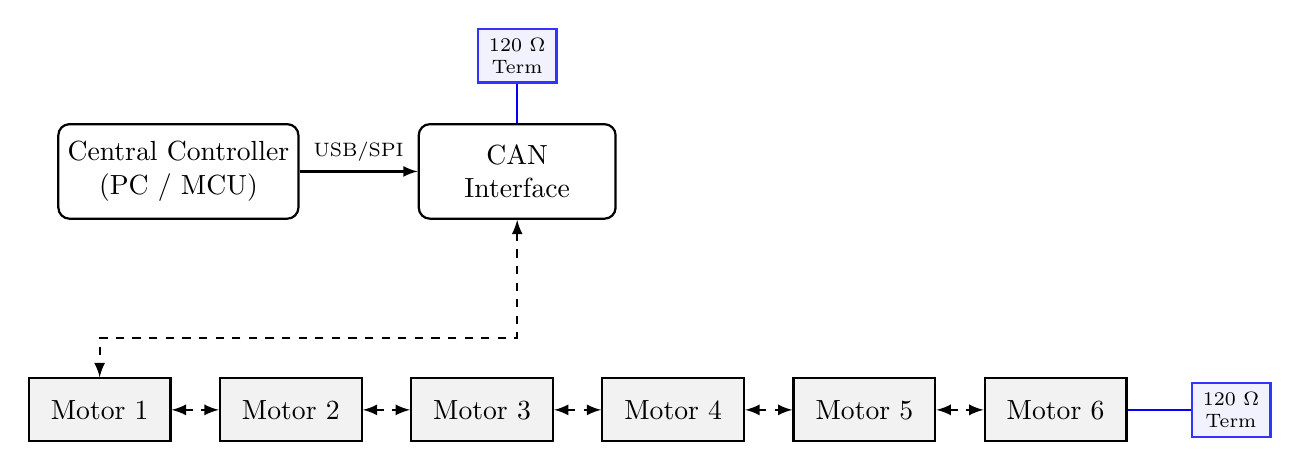
\begin{tikzpicture}[
    node distance=1.5cm,
    box/.style={rectangle, draw=black, rounded corners, align=center, minimum width=2.5cm, minimum height=1.2cm, thick, fill=white},
    motor/.style={rectangle, draw=black, align=center, minimum width=1.8cm, minimum height=0.8cm, thick, fill=gray!10},
    line/.style={draw, thick, -latex},
    canline/.style={draw, thick, dashed, latex-latex},
    resistor/.style={rectangle, draw=blue!80, thick, fill=blue!5, align=center, minimum width=1cm, minimum height=0.5cm, font=\scriptsize}
]

% Nodes
\node[box] (pc) {Central Controller\\(PC / MCU)};
\node[box, right=1.5cm of pc] (can) {CAN\\Interface};

\node[motor, below=2cm of pc, xshift=-1cm] (m1) {Motor 1};
\node[motor, right=0.6cm of m1] (m2) {Motor 2};
\node[motor, right=0.6cm of m2] (m3) {Motor 3};
\node[motor, right=0.6cm of m3] (m4) {Motor 4};
\node[motor, right=0.6cm of m4] (m5) {Motor 5};
\node[motor, right=0.6cm of m5] (m6) {Motor 6};

% Termination Resistors
\node[resistor, above=0.5cm of can] (r1) {$120~\Omega$\\Term};
\node[resistor, right=0.8cm of m6] (r2) {$120~\Omega$\\Term};

% Connections
\draw[line] (pc) -- node[above, font=\scriptsize] {USB/SPI} (can);
\draw[thick, blue] (can.north) -- (r1.south);
\draw[thick, blue] (m6.east) -- (r2.west);

% CAN Bus Daisy Chain
\draw[canline] (can.south) |- ([yshift=0.5cm]m1.north) -- (m1.north);
\draw[canline] (m1.east) -- (m2.west);
\draw[canline] (m2.east) -- (m3.west);
\draw[canline] (m3.east) -- (m4.west);
\draw[canline] (m4.east) -- (m5.west);
\draw[canline] (m5.east) -- (m6.west);

\end{tikzpicture}
\caption{CAN Bus daisy-chain communication topology featuring standard $120~\Omega$ termination resistors to ensure signal integrity.}
\end{figure}

\subsection{Software Protocol and Actuation}
At the software level, the controller communicates with the MyActuator drivers by transmitting standard CAN frames. Each frame consists of a specific CAN ID (targeting an individual motor axis), a Data Length Code (DLC, typically 8 bytes), and a Data Payload containing the precise hexadecimal commands for position, velocity, and current limits. 

\noindent
To achieve smooth, multi-axis coordinated movement, the software executes a real-time control loop (operating between 100Hz and 500Hz). In each cycle, the controller calculates the inverse kinematics, broadcasts the target position frames to all six axes, and receives immediate feedback frames detailing the current physical angle and electrical current draw of each motor.

\end{document}